\ifx\headerIncludedJR\undefined
  \documentclass[11pt,a4paper]{article}
  \setlength{\textwidth}{5.50in}
  \usepackage[utf8]{inputenc}
\usepackage[T1]{fontenc}
\usepackage{amsmath}
\usepackage{amsthm}
\usepackage{amssymb}
%\usepackage{rotating}
%\usepackage{amslatex}
\usepackage{siunitx}
\usepackage{multicol}%for multicol
\usepackage{blkarray}%blockarray and block
\usepackage{comment}
\usepackage{fnbreak}%get a warning if a footnote is split
\usepackage[section]{placeins}
\usepackage{listings}
\lstset{breaklines=true,basicstyle=\ttfamily,language=Python}
\usepackage{arrayjobx}
\usepackage{array}%for \newcolumntype
%\usepackage[shortlabels]{enumitem}
\usepackage{mathtools}
\usepackage{afterpage}
\usepackage{setspace}% for \setstretch
\usepackage{algorithm}
\usepackage{algpseudocode}%for algorithmic
\usepackage{thmtools}%so that autoref works with Lemmas
\usepackage{tikz}
\usepackage{pgfplots}
\pgfplotsset{compat=1.15}
\usepackage{shuffle}
\usepackage{textcomp}%for \textrecipe
\usepackage{fontawesome}%for \faTable
\usetikzlibrary{calc,shapes,arrows.meta,decorations.markings,arrows}
\usetikzlibrary{graphs,positioning,svg.path,backgrounds}
\newcommand{\tikzmark}[1]{\tikz[overlay,remember picture] \node (#1) {};}
%\usepackage{CJKutf8}%for CJKChar

%\usepackage[backend=biber,backref=true]{biblatex}
\usepackage[backend=biber,style=alphabetic,backref=true,maxbibnames=10]{biblatex}
\addbibresource{sigs.bib}
\usepackage{url}

\usepackage{imakeidx}
%not a list of definitions, just symbols and abbreviations
%What is an abbreviation? Is QR? 
\makeindex[intoc,title=Symbols and abbreviations index]
\def\jind#1{\index{#1}}
\def\jindmath#1#2{\index{#2@$#1$}}
\def\jindv#1{\index{#1v@\texttt{#1}}}
%Some places I've given up and used \index in the text 
\definecolor{bluee}{rgb}{0.4, 0.4, 1.0}
%https://tex.stackexchange.com/questions/134191/line-breaks-of-long-urls-in-biblatex-bibliography
\setcounter{biburlucpenalty}{8000}
\setcounter{biburllcpenalty}{8000}

\usepackage{hyperref}

%so that autoref works with algorithms
\newcommand{\algorithmautorefname}{Algorithm}

%might help url breaking in bibliography
%\Urlmuskip=0mu plus 1mu minus 1mu
%also all the emergencystretch/looseness/fussy/sloppy
%to play with
%https://tex.stackexchange.com/questions/18505/how-to-use-sloppy-for-just-some-references

\def\ii{{\texttt{iisignature}}}
\def\pypi{{\texttt{PyPI}}}
\def\numpy{{\texttt{numpy}}}
\def\scipy{{\texttt{scipy}}}
\def\i#1{\index{#1@\texttt{#1}}}
\def \hilite#1{\underline{\color{blue}\textbf{#1}}}
%\def \alph#1{{\color{blue}\mathbf{#1}}}
\def \lex{<_L}
\def\kron{\underline{\otimes}}

\graphicspath{{C:/Users/Jeremy/Dropbox/phd/graphs/}{/home/jeremyr/Dropbox/phd/graphs/}{/Users/reizenstein/DropboxPersonalSymlink/phd/graphs/}}

%\RequirePackage{relsize}
%\DeclareRobustCommand\CXX{C\kern-.05em \raisebox{.3ex}{\scalebox{0.9}{\textbf{+\kern-.10em+}}}}
\DeclareRobustCommand\CXX{C\kern-.05em {\scalebox{0.9}{\textbf{+\kern-.10em+}}}}
%\DeclareRobustCommand\{\texorpdfstring{\CXX}{C++}}
\DeclareRobustCommand\CC{C\texttt{++}}
\def\bftab{\fontseries{b}\selectfont}
\newtheorem{theorem}{Theorem}
%\newtheorem*{theorem*}{Theorem}%bad idea, because you can't refer to it.
\newtheorem{definition}[theorem]{Definition}
%\newtheorem{outsideTheorem}[theorem]{Theorem}
\newtheorem{example}[theorem]{Example}
\newtheorem{conjecture}[theorem]{Conjecture}
\newtheorem{lemma}[theorem]{Lemma}
\newtheorem{proposition}[theorem]{Proposition}
\newtheorem{remark}[theorem]{Remark}

\newcommand{\area}{\mathsf{area}}
\newcommand{\Area}{\mathsf{Area}}
\newcommand{\emptyword}{\epsilon}
\newcommand{\ds}{d} % dimension of the signal
\newcommand{\TC}{T((\R^\ds))} % concat
\newcommand{\TS}{T(\R^\ds)} % shuffle
\newcommand{\GL}{\operatorname{GL}}
\newcommand{\SO}{\operatorname{SO}}
%\newcommand{\id}{\operatorname{id}}
\newcommand{\id}{\mathsf{id}}

\newcommand{\evaluatedAt}[1]{\,\raisebox{-.5em}{$\vert_{#1}$}}

\def\hssymbol{\mathbin{\succ}}
\def\hs#1#2{#1\hssymbol#2} %half shuffle
%\def\hs#1#2{z(#1,#2)} %half shuffle
\def\areab#1{\underline{\area}(#1)}
\def\areabb{\underline{\area}}
\newcommand{\R}{\mathbb{R}}
\newcommand{\Q}{\mathbb{Q}}
\newcommand{\C}{\mathbb{C}}
\newcommand{\N}{\mathbb{N}}
\newcommand{\spann}{\operatorname{span}}
\newcommand{\sign}{\operatorname{sign}}

\DeclareMathOperator*{\argmax}{arg\,max}
\DeclareMathOperator*{\argmin}{arg\,min}
\DeclareMathOperator{\softmax}{softmax}

%indicate that this file has been had
\def\headerIncludedJR{}
\def\endDocumentJR{}

%general hints
%https://homepages.inf.ed.ac.uk/imurray2/compnotes/latex.html

  %this cannot be in header.tex as it messes up
  %the thesis copyright page
  \def \alph#1{{\color{bluee}\mathbf{#1}}}
  \begin{document}
  \tableofcontents
  \def\endDocumentJR{\printindex \printbibliography[heading=bibintoc]\end{document}}
\fi

\section{Tools}
Here I describe a number of new software tools for examining the signature which I have found useful, and which should help people in different ways trying to get to know the signature and its behaviour. They are not all original ideas.
\subsection{Five points in two dimensions}
\begin{figure}
	\begin{center}
		\includegraphics[width=0.8\textwidth]{MathematicaView2.png}
	\end{center}
	\caption[The \texttt{view.m} tool showing a path among five points.]{\label{fig:MathematicaView}The \texttt{view.m} tool showing a path among five points. The widgets on the right show its log signature up to level 8.}
\end{figure}
In the specific case $d=2$, $m=4$, the log signature has eight components, and a two dimensional path with four segments has eight degrees of freedom. The file \verb|view.m| provides an interactive Mathematica~10 visualisation of the relationship between a path made of four segments and its log signature. It depends on another file \verb|bch.m|, which has been generated by additional functionality in the original python logsignature code \cite{LOGSIG}, which defines a single function returning the log signature of a path defined by four displacements. The visualisation should appear when \verb|view.m| is run. The log signature appears as widgets on the right of the graph of the path. Because level 1 and level 3 of the log signature are two dimensional, they are represented by 2d controls. The other log signature components are controlled separately. When `solve' is ticked, you can gently move the widgets to change the components of the log signature and see the path move. Note that the $\alph{12}$ component controls the signed area enclosed by the path. The calculation of solutions is not perfect, but is enough to get a general picture. It is relying on built-in nonlinear optimisation routines in Mathematica to attempt to invert the signature in this special case.
%TODO: this should use polynomial methods instead. see the Polynomial Systems guide
When `solve' is unticked, you can drag the locators to change the path, and see the corresponding log signature elements move. For example, after drawing 3 paths the window might look as shown in \autoref{fig:MathematicaView}.

\subsection{Freehand drawing}
The simple tool \verb|freehand_draw.py| lets you draw paths with your mouse in a blank window. The signature of each path is printed on the console. This is one tool I wanted to have in order to get a feel for the signature elements. Signed area and its robustness on paths which are nearly closed is particularly easy to illustrate with the tool.

For example, after drawing 3 paths the window might look as shown in \autoref{fig:hey}.
\begin{figure}
%	\includegraphics[trim=0pt 10pt 0pt 0pt, clip,width=0.8\textwidth]{hey.gif}
\begin{center}
	\includegraphics{hey.png}
\end{center}
\caption{\label{fig:hey}Appearance of \texttt{freehand\char`_draw.py} after some mouse drags.}
\end{figure}
The following would be printed on the console, indicating truncated log signatures up to level 3 of each path. In particular, the three lines in order correspond to (1) the letters of the word `hey', (2) the vertical stroke of the exclamation mark and (3) the dot.
%\begin{quotation}
\begin{lstlisting}
[ 0.366492 -0.379581  0.020182 -0.007912 -0.003532]
[-0.002618 -0.212042  0.001631 -0.000008 -0.000014]
[ 0.002618  0.005236  0.000154  0.000001  0.000001]
\end{lstlisting}
%\end{quotation}

\subsection{Arbitrary precision signature calculations}
The \ii\ project sources include a project \verb|arbprec| which calculates signatures of paths in arbitrary precision and compares them to those using floating point arithmetic. Very often we see that these results do not differ by much for random paths. There are cases where calculating the signature of a path naturally results in a loss of floating point accuracy, for example the 1-dimensional path $(0),(a),(b)$ where $a\approx1$ and $b\approx0$, and so testing with arbitrary precision may be useful.
Long paths given by lots of points could create a unique problem, with this type of cancellation happening in some dimensions.
%Could illustrate this in mathematica with a long path that backtracks

\subsection{Free lie algebra calculations}

The file \verb|free_lie_algebra.py|\footnote{\url{github.com/bottler/free-lie-algebra-py}} provides objects to do many of the calculations described in \cite{FLA}. The main types are summarised in \autoref{tab:flaTypes}. It is useful for getting intuition and testing out conjectures, and is generally hackable.

As an example, we could try to find the linear combination of signature elements corresponding to the coefficient of $\alph{112}$ in the log signature in the Lyndon basis. We might do that like this using the method of \autoref{sec:usepi1adjoint}.
\begin{quotation}
\begin{lstlisting}[language=Python]
from free_lie_algebra import *
d=2
m=3
H=HallBasis(d,m,lessExpressionLyndon)

with UseRationalContext():
    answer=pi1adjoint(S("112",H))
\end{lstlisting}
\end{quotation}
This sets \verb|answer| to the \verb|Elt| representing $\pi_1^\top(S_{\alph{112}})$ which is what we are looking for.
If we run \lstinline[language=Python]{print(answer.pretty())} we will be told 
\begin{quotation}
	\begin{lstlisting}
	[1/6]112-[1/3]121+[1/6]211
	\end{lstlisting}
\end{quotation}
which fits with what we would come up with by staring at \eqref{eq:arbsig} to find a (in fact, the \emph{unique}) linear combination of elements which adds up to $d$, namely that
\begin{align*}
\def\b{\Big}
d=\frac16\b(\frac{a^2b+6d+3ac}{6}\b)-\frac13\b(\frac{a^2b-12d}{6}\b)+\frac16\b(\frac{a^2b+6d-3ac}{6}\b).
\end{align*}
%Without \verb|UseRationalContext|, the library uses its floating point numbers as the coefficients, which is less pretty.
The library uses floating point numbers as coefficients by default. The use of \verb|UseRationalContext| makes it use rational numbers from \verb|sympy| \cite{sympy}, which is prettier in a case like this.

We can further verify this in the code. The \verb|arbitraryGrouplikeEltSympy| function returns an arbitrary truncated signature expression as an \verb|Elt| in the style of \eqref{eq:arbsig}.
The coefficients are \verb|sympy| expressions. 
It is a tensor where each element in terms of its corresponding log signature elements for a given Hall basis.
Instead of labelling the log signature elements with letters of the alphabet like the $a,b,c,\dots$ of \eqref{eq:arblogsig}, the element corresponding to a word is given a name \verb|x| subscripted with the number which looks like the word. For example $c$ is \verb|x_12|.
We can perform the verification like this
\begin{quotation}
\begin{lstlisting}[language=Python]
    sig = arbitraryGrouplikeEltSympy(H)
    print(dotprod(sig,answer).expand())
\end{lstlisting}
\end{quotation}
which prints \verb|x_112| as desired.

%The alphabet $A$ is \verb|int| starting from 1. %The scalars are \verb|int| or \verb|float|, but this is made easy to change. The main types are listed in Table~\ref{tab:flaTypes}. Addition and scalar multiplication are overloaded, and the other main functions in Table~\ref{tab:flaOps}. The \verb|test()| function serves as a demonstration.
\begin{table}
\begin{tabular}{lp{3.4in}}
%\begin{tabular}{ll}
name&set\\%&comment\\
\hline
\verb|Word|&$\Sigma^*$\\
\verb|Elt|&tensor space, $K\langle \Sigma\rangle$\\
\verb|EltElt|&$K\langle \Sigma\rangle^{\otimes n}$, any $n$\\
\verb|tuple(int...)|&free magma, $M\langle \Sigma\rangle$\\
\verb|HallBasis|&a Hall basis for a given dimension and depth/level.\\
\verb|TensorSpaceBasis|&a basis of $K\langle \Sigma\rangle$, e.g.~the PBW basis or its dual, up to a given dimension and depth/level.
\end{tabular}
\caption{\label{tab:flaTypes}Types in \texttt{free\symbol{95}lie\symbol{95}algebra.h}}
\end{table}
\iffalse
\begin{table}
\begin{tabular}{lll}
function name&\pbox{2.4cm}{mathematical\\symbol}&comment\\\hline
\verb|concatenate|&&(concatenate words)\\
\verb|concatenationProduct|&&(concatenation product of \verb|Elt|)\\
\verb|concatenationProductEltElt|&&(concatenation product of \verb|EltElt|)\\
\verb|shuffleProduct|&$\shuffle$\\
\verb|tensorProduct|&$\otimes$\\
\verb|tensorProductFunctions|&$f_1\otimes f_2\otimes\dots$&where $f_i:\verb|Elt|\to\verb|Elt|\;\mathrm{or}\;\verb|EltElt|$\\
\verb|lieProduct|&$[\cdot,\cdot]$\\
\verb|dotprod|&&inner product of \verb|Elt| in basis of words\\
\verb|distance|&&distance between \verb|Elt|s in basis of words\\

\verb|conc|&conc and $\mathrm{conc}_p$\\
\verb|sh|&sh\\
\verb|sh_p|&$\mathrm{sh}_p$\\
\verb|epsilon|&$\varepsilon$&constant term of tensor\\
\verb|delta|&$\delta$&adjoint of sh\\
\verb|deltabar|&$\bar\delta$\\
\verb|deltadash|&$\delta'$&adjoint of conc\\
\verb|lambda_|&$\lambda$\\
\verb|mu|&$\mu$\\
\verb|star|&$*$\\
\verb|stardash|&$*'$\\
\verb|r|&$r$&right bracketing: $r(\alph{123})=[\alph1,[\alph2,\alph3]]$\\
\verb|alpha|&$\alpha$&antipode, inverse under concatenation product\\
\verb|log1p|&$\log(1+\cdot)$\\
\verb|log|&$\log$\\
\verb|exp|&$\exp$\\
\verb|Ad|&Ad\\
\verb|ad|&ad\\
\verb|id|&id&identity function on \verb|Elt|\\
\verb|D|&$D$\\
\verb|P|&$P_\cdot$&PBW basis element of a word\\
\verb|S|&$S_\cdot$&PBW dual basis element\\
\verb|Q|&$Q_\cdot$&shuffle of Lyndon factors\\
\end{tabular}
\caption{\label{tab:flaOps}Functions in \texttt{free\symbol{95}lie\symbol{95}algebra.h}}
\end{table}
\fi

\subsection{Mathematica signature tools}
Mathematica has a highly regarded system for symbolic integration. If someone has a curve given in mathematical form and wants to try to calculate its signature in closed form or numerically, it would make sense to use Mathematica. Therefore I created tools to make this easy.

\verb|parametricCurves.wl| provides functions for manipulating parametric curves (which are represented either as a list of functions or a list of expressions). Some simple manipulations are provided (shifting, concatenating, plotting, adding a time dimension) which may be useful for experiments. The calculation of the signature, with iterative calls to Mathematica's integrator, is the main capability.
For example, a calculation of the signature of one revolution of a circle up to level 3 could be requested with
\begin{quotation}
	\begin{lstlisting}
	SigFns[{Cos, Sin}, 2 Pi, 3]
	\end{lstlisting}
\end{quotation}
which results in the following.
\begin{quotation}
	\begin{lstlisting}
{{0, 0}, 
 {{0, Pi}, {-Pi, 0}}, 
 {{{0, -Pi}, {2*Pi, 0}},{{-Pi, 0}, {0, 0}}}}
	\end{lstlisting}
\end{quotation}

\verb|bases.wl| contains basic Hall basis calculations sufficient to map an expanded log signature to a basis. This is expressed in a way close enough to the mathematical presentation to be instructive.
\verb|calcSignature.wl| calculates signatures and log signatures of piecewise linear curves using straight Mathematica code. 
This is like the basic functionality of \verb|iisignature|. This is again instructive rather than intended to be used for high volume calculation.
I similarly provided examples of the basic calculation of the signature of a path through given points in \texttt{R} and \texttt{matlab} because people ask.

%\section{Tricks and tips}

%PROPERTIES Document

\section{A conjecture about figures of eight}
%? (?Hector) Sussman had a plan for inverting the sig using paths which vanish up to each level.
One way I attempted to get a feel for signature elements is to think about paths which are simple and whose signatures are zero up to a certain level. This is something that has been considered for example in \cite{Gauthier}.
%TERMINOLOGY STEP-N SIGNATURE
%TODO - merge with text from properties file
In section~7.5.2 of \cite{FrizVictoir} it is shown that among paths whose signature is a given truncated grouplike element, equivalently among all the paths with a given truncated log signature, there is a unique shortest path and it can be parameterised at constant speed. %in a Lipschitz continuous way..
Finding it for a given truncated signature, or indeed any path, is an open problem in general.
For level 1, this path is a straight line.
For level 2 given, it is quite easy to find the path, it will be a piece of circle or helix. This follows from the work in \cite{BrockettDai}.
There is no easy way to find the path for higher levels, although this would be quite informative.
For level 3, a numerical attempt has recently been announced in \cite{AnnaInverting}.
Having paths which are zero up to each level could be useful not only for gaining intuition but also because they could be combined to produce paths which agree with a given signature.
In this section, I present an interesting pattern which looks like a supply of paths whose first non-zero signature level is arbitrarily high.
 %Finding any path with a given truncated signature is the problem of ``inverting the signature'', which is a research topic.

In electromagnetism, it is common to consider a dipole moment, the long-range effect of two nearby particles of opposite charge.
Magnetic poles come in pairs in nature, and we often consider combinations of them in such a way that the total dipole moment is zero, leading us to quadrupole moments. The process continues.
The fact that a figure of eight has nonzero values in level 3 of its signature but zero values in level 1 and 2, which is seen because it is closed and the areas of each loop (which have signed area but no displacement) come with opposite signs, is reminiscent of this process.

By numerical experiment, I have found a pattern where traversing a figure of eight several times (all starting from the central crossing point) I can get paths whose signatures are zero up to many levels. There are four ways to traverse a given figure of eight with zero area -- just by choosing which direction to start. 

\begin{figure}
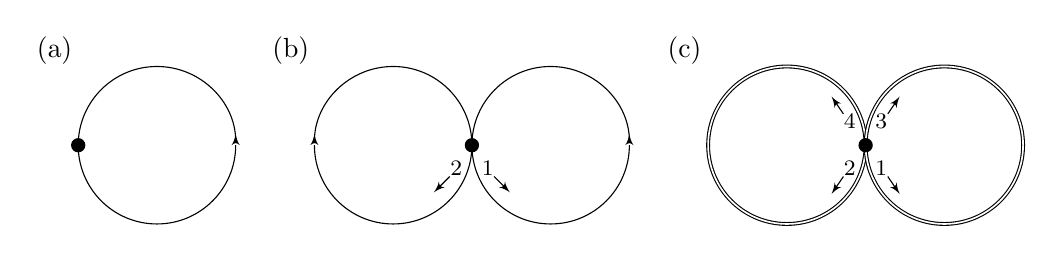
\begin{tikzpicture}
%\begin{scope}[decoration={ %very thick?  thick?
%  markings,
%  mark=at position 0.5 with {\arrow[xshift=2mm]{Latex[length=4mm,width=2mm]};}}
%] 
%\draw[->,>=latex'] (0,0) arc[radius=1,start angle=0,delta angle=360];
%\node[minimum height=1.2ex,inner sep=0pt,circle,fill=black,label=right:start/end]at (2,0){};
\node at (-0.3,1.2) {(a)};
\draw[>-,>=latex'] (2,0) arc[radius=1,start angle=0,delta angle=360];
\node[minimum height=1.2ex,inner sep=0pt,circle,fill=black]at (0,0){};
%\node at (0,0) {d};
%\end{scope}
\begin{scope}[xshift=3cm]
\node at (-0.3,1.2) {(b)};
\draw[-<,>=latex'] (0,0) arc[radius=1,start angle=180,delta angle=360];
\draw[>-,>=latex'] (4,0) arc[radius=1,start angle=0,delta angle=360];
\node[minimum height=1.2ex,inner sep=0pt,circle,fill=black]at (2,0){};
\node [inner sep=0](x1) at (2.2,-0.3) {\footnotesize 1};
\node [inner sep=0](x2) at (1.8,-0.3) {\footnotesize 2};
\draw [-latex'](x1.south east) -> ++(0.2,-0.2);
\draw [-latex'](x2.south west) -> ++(-0.2,-0.2);
\begin{scope}[xshift=5cm]
\node at (-0.3,1.2) {(c)};
\draw[double](0,0) arc[radius=1,start angle=180,delta angle=360];
\draw[double](4,0) arc[radius=1,start angle=0,delta angle=360];
\node[minimum height=1.2ex,inner sep=0pt,circle,fill=black]at (2,0){};
\node [inner sep=0](x1) at (2.2,-0.3) {\footnotesize 1};
\node [inner sep=0](x2) at (1.8,-0.3) {\footnotesize 2};
\node [inner sep=0](x3) at (2.2,0.3) {\footnotesize 3};
\node [inner sep=0](x4) at (1.8,0.3) {\footnotesize 4};
\draw [-latex'](x1.south east) -> ++(0.15,-0.22);
\draw [-latex'](x2.south west) -> ++(-0.15,-0.22);
\draw [-latex'](x3.north east) -> ++(0.15,0.22);
\draw [-latex'](x4.north west) -> ++(-0.15,0.22);
\end{scope}
\end{scope}
\end{tikzpicture}
\caption[First curves in the figure 8 Fibonacci pattern.]{\label{fig:fibonacci}Closed paths are shown with their start and end marked with a solid circle.
(a) A circle, a path whose first nonzero signature entry is on level 2.
(b) A figure of eight made of two circles, a path whose first nonzero signature entry is on level 3.
(c) A path made of two traverses of the same figure of eight, whose first nonzero signature entry is on level 5.}
\end{figure}

\begin{figure}
	\centering
	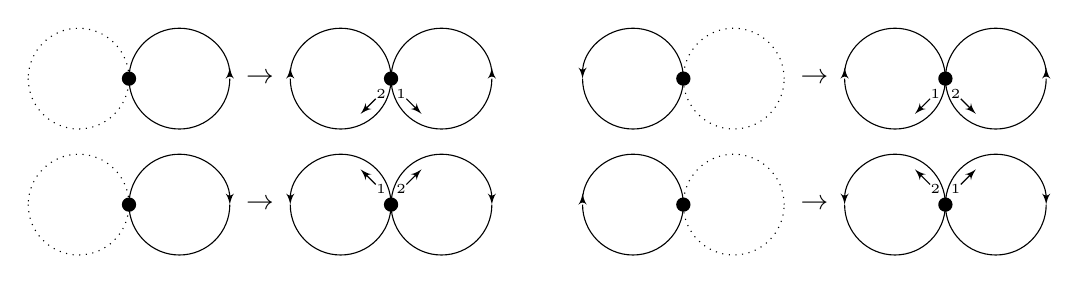
\begin{tikzpicture}[scale=0.64]
	\def\vertsep{2.5cm}
	\def\horsep{11cm}
	\def\radius{1}
	\def\tworadius{2}
	\def\fourradius{4}
	\def\aplus#1{\ifodd#1 +\else-\fi}
	\def\aminus#1{\ifodd#1 -\else+\fi}
	%\def\aminus#1{-}
	\def\asouth#1{\ifodd#1 south\else north\fi}
	\def\aeast#1{\ifodd#1 east\else west\fi}
	\def\awest#1{\ifodd#1 west\else east\fi}
	\def\al#1{\ifodd#1 <\else >\fi}
	\def\ar#1{\ifodd#1 >\else <\fi}
	\def\a#1#2#3#4{
		\draw[#1,>=latex'] (0,0) arc[radius=\radius,start angle=180,delta angle=360];
		\draw[#2,>=latex'] (\fourradius,0) arc[radius=\radius,start angle=0,delta angle=360];
		\node[minimum height=1.2ex,inner sep=0pt,circle,fill=black]at (\tworadius,0){};
		\node at (4.6cm,0) {$\to$};
		\begin{scope}[xshift=5.2cm]
		\draw[-\al{#3},>=latex'] (0,0) arc[radius=\radius,start angle=180,delta angle=360];
		\draw[\ar{#3}-,>=latex'] (\fourradius,0) arc[radius=\radius,start angle=0,delta angle=360];
		\node[minimum height=1.2ex,inner sep=0pt,circle,fill=black]at (\tworadius,0){};
		\node [inner sep=0](x1) at ($(2,\aminus{#3}0.3)+(\aplus{#4}0.2,0)$) {\tiny 1};
		\node [inner sep=0](x2) at ($(2,\aminus{#3}0.3)+(\aminus{#4}0.2,0)$) {\tiny 2};
		\draw [-latex'](x1.{\asouth{#3} \aeast{#4}}) -> ++(\aplus{#4}0.3,\aminus{#3}0.3);
		\draw [-latex'](x2.{\asouth{#3} \awest{#4}}) -> ++(\aminus{#4}0.3,\aminus{#3}0.3);
		\end{scope}
	}
	\a{dotted}{>-}11
	\begin{scope}[yshift=-\vertsep]
	\a{dotted}{<-}00
	\end{scope}
	\begin{scope}[xshift=\horsep]
	\a{->}{dotted}10
	\begin{scope}[yshift=-\vertsep]
	\a{-<}{dotted}01
	\end{scope}
	\end{scope}
	\end{tikzpicture}
\caption[The general step in the figure 8 Fibonacci pattern.]{\label{fig:fibonacciPattern}The transformation of each loop in the path to a figure of 8 which leads from each path to the next.}
\end{figure}
\begin{itemize}
\item Two such figure-of-eight traverses can be concatenated to a path which makes a total of four loops whose first nonzero signature elements are at level 5. These paths are shown in \autoref{fig:fibonacci}.
\item Two such four-loop traverses can be concatenated (in exactly one way) to make a path which has 8 loops and whose first nonzero signature elements are at level 8.
\item Two such 8 loop traverses can be concatenated (in exactly one way) to make a path which has 16 loops and whose first nonzero signature elements are at level 13.
\item Two such traverses can be concatenated in exactly one way to make a path whose signature is zero up to at least level 18.
\end{itemize}
The general process which goes from one of these paths to the next is that of replacing each single loop by a figure of eight in the pattern shown in \autoref{fig:fibonacciPattern}. This pattern is reminiscent of the way the Thue-Morse sequence is generated. For example, the pattern of whether each loop is clockwise or anticlockwise in one of these paths corresponds to the Thue-Morse sequence.
Calculating signatures for these paths is illustrated in the file \verb|figure8Fibonacci.py| which uses \verb|iisignature| to calculate signatures. 
%It is hard to visualise these paths in a nice way. 
It is simple to conjecture that paths can be formed in this way whose first nonzero signature elements are any given Fibonacci number.


\endDocumentJR
